\documentclass[
    11pt,               % KOMA default
    a4paper,            % DIN A4
    %twoside,            % Zweiseitig
%     onside,
    headsepline,        % Linie unter der Kopfzeile
    foodsepline,        % Linie �ber Fussnote
    %automark,           % Kolumnentitel lebendig
    %pointlessnumbers,   % Keinen Punkt hinter die letzte Zahl
                        % eines Kapitels (auch bei Anhang)
%     openleft,           %
    %openright,
    cleardoubleplain,   %
    %abstracton,         %
    %idxtotoc,           % Index soll im Inhaltsverzeichnis auftauchen
    liststotoc,         %
    bibtotoc,           %
    %parskip            % parskip-, parskip*, parskip+
]%{scrreprt}
{scrartcl}

%\usepackage[latin1]{inputenc}
\usepackage[utf8]{inputenc}
\usepackage[ngerman]{babel}
\usepackage{graphicx}
\usepackage{subfigure}
\usepackage{float}
\usepackage{listings}
\usepackage{color}
\usepackage{tabularx}
\usepackage[hidelinks]{hyperref}
\usepackage{tabu}
\usepackage{booktabs}
\usepackage[table]{xcolor}
\usepackage{url}
\usepackage{lmodern}
\usepackage{amsmath}
\usepackage{amsfonts}
\usepackage{amssymb}

% Definitions
\definecolor{mydarkblue}{rgb}{0.0,0.0,0.5}
\definecolor{mylightblue}{rgb}{0.85,0.85,0.85}
\definecolor{mylightgray}{rgb}{0.95,0.95,0.95}

\newcommand{\HRule}{\rule{\linewidth}{0.4mm}}

\clubpenalty=10000
\widowpenalty=10000

\begin{document}

%\newpage
\pagestyle{empty}
\begin{center}
	
\includegraphics[scale=0.8]{images/hszg_logo.png}\\
	\vspace*{2cm}
	%\Large
	%\textbf{Fakultät}\\
	%\textbf{Elektrotechnik und Informatik}\\
	%\vspace*{2cm}
	\Huge
	\textbf{Belegarbeit}\\
	\Large
	\vspace*{2cm}
	\textbf{Analyse und Bewertung von Tools als Ersatz für das BSI-GS-Tool}\\
	\vspace*{1cm}
	
	\vfill
	\normalsize
	\newcolumntype{x}[1]{>{\raggedleft\arraybackslash\hspace{0pt}}p{#1}}
	\begin{tabular}{x{6cm}p{7.5cm}}
		\rule{0mm}{5ex}Kucera, Adam & {Matr.-Nr.:} 202549\\
		\rule{0mm}{5ex}Krause, Andre & {Matr.-Nr.:} 46932\\
		\rule{0mm}{5ex}Leuschner, Jens & {Matr.-Nr.:} 200479\\
		\rule{0mm}{5ex}Mack, Tobias & {Matr.-Nr.:} 209865\\
		\rule{0mm}{5ex}Michel-Suarez, Maria Belen & {Matr.-Nr.:} 209782\\
		\rule{0mm}{5ex}Müssig, Daniel & {Matr.-Nr.:} 200304\\
		\rule{0mm}{5ex}Riedel, Robert & {Matr.-Nr.:} 202349\\
		\rule{0mm}{5ex}Wollstein, Romano & {Matr.-Nr.:} 200616\\
		\rule{0mm}{5ex}Zoeke, Robert & {Matr.-Nr.:} 200074\\

		\rule{0mm}{5ex}\textbf{Abgabedatum:} & 02.02.2015 \\ 
	\end{tabular} 
\end{center}
%\section*{Abstract}

\pdfbookmark{\contentsname}{toc}\tableofcontents
\thispagestyle{empty}

\newpage
\pagestyle{empty}
\listoffigures

\newpage
\listoftables

\newpage
\pagestyle{plain}
\setcounter{section}{0}
\pagenumbering{arabic}

\subsection{Aufteilung}
Die Aufgaben innerhalb der Gruppe wurden wie folgt aufgeteilt:

\begin{table}[H]
	\sffamily
	\caption{Aufgabenverteilung}
	\tabulinesep = 1mm %bringt die Reihen etwas weiter auseinander, angenehmer zu lesen
	\centering
		\begin{tabu} to 0.9\textwidth { X[1.7]  X[3] }
		\hline
		\textbf{Name} & \textbf{Aufgabe}\\
		\hline 
		Kucera, Adam & TODO\\

		Krause, Andre & Doc SetMinder, HiScout, GRC Suite iRIS, opus i\\

		Leuschner, Jens & TODO\\

		Mack, Tobias & AttackTrees\\

		Michel-Suarez, Maria Belen & Crisam\\

		Müssig, Daniel & SAVe - Security Audit and Verification\\

		Riedel, Robert & Koordination, Sidoc, Beschreibung der Kriterien\\

		Wollstein, Romano & TODO\\

		Zoeke, Robert & Einleitung, Aufgabe, Indart, Bsp-HS,DNC Vision\\

	\end{tabu}
\end{table}

Der IT-Grundschutz existiert seit 20 Jahren. Im Rahmen dieses Jubiläums hat das BSI beschlossen eine Optimierung und Aktualisierung der Vorgehensweise und IT-Grundschutz-Kataloge durchzuführen\cite{bsi}. Das BSI setzt sich die folgenden Ziele. Man will dem Bedarf der Anwender mit einem stets aktuellen und praxisnahen Verfahren gerecht werden. Dazu ist es auch wichtig, die Kontinuität zu gewährleisten und die alte IT-Grundschutz Welt weiterzuentwickeln. Das Ziel ist es hauptsächlich die Attraktivität zu erhöhen und den Weg für die nächsten 20 Jahre zu bereiten.

Die Toolunterstützung wird dabei als unabdingbar angesehen. Ein Tool kann dabei auch ein Wiki oder Ähnliches sein. Das Wichtigste ist eine gute Akzeptanz im Unternehmen, damit das Tool nicht ungenutzt bleibt. Es kommt alles in Frage, was die Arbeit mit dem IT-Grundschutz vor, während und nach einer Zertifizierung erleichtert und unterstützt.

\subsection{Aufgabenstellung}
An der Fachhochschule Görlitz wird für Lehrveranstaltungen zur Informationssicherheit und zum
Informationssicherheitsmanagement zurzeit das GSTOOL des BSI eingesetzt. Da die Weiterentwicklung dieses Tools eingestellt wurde und es in der Lehre wichtig ist aktuell zu bleiben, ist nach einer Alternative für den Einsatz in der Lehre zu suchen. 
Weiterhin ist es an der Hochschule dringend nötig, ein IT-Sicherheitskonzept zu erstellen und umzusetzen. Daher ist auch die Frage nach einem dafür geeigneten Tool zu klären. 

Dieses Projekt hat das Ziel Bewertungskriterien, sowohl für die Lehre, als auch den produktiven Einsatz an der Hochschule, auszuarbeiten, die von einem geeigneten Tool erfüllt werden müssen. Diese Bewertungskriterien sind auf die auf der Webseite des BSI genannten Alternativtools anzuwenden um einen Entscheidungsvorschlag zu erarbeiten.

\section{Bewertungskriterien}
Um alle untersuchten Programme einheitlich miteinander vergleichen zu können, wurde eine Liste von Bewertungskriterien erarbeitet, welche im folgenden kurz erklärt werden soll.\\
Die Bewertungsskala reicht von 0 bis 10, in aufsteigender Wertigkeit. Soweit nicht gesondert erwähnt, wird ein Merkmal mit 0 gewertet, wenn es nicht vorhanden ist und mit 10, wenn es wirklich gut ausgearbeitet ist.\\
Um die abschließende Wertung für den Einsatz in der Hochschule bzw. in der Lehre zu ermitteln, werden die Rohwertungen in einer Kategorie mit einer Gewichtung multipliziert, welche Tabelle ~\ref{tab:gewichtung} zu entnehmen ist. Die Gesamtwertung wird dann prozentual von der maximal möglichen Punktzahl angegeben.
\begin{itemize}
	\item \textit{Wizard} bewertet, ob es eine Führung durch das Programm mittels Wizards gibt und wie gut diese umgesetzt ist. 10 = gut umgesetzte benutzerfreundliche Wizardführung durch alle wichtigen Programmaspekte.

	\item \textit{Infrastrukturdarstellung} bewertet, wie umfangreich und übersichtlich die modellierten Komponenten Dargestellt werden.

	\item \textit{Netzpläne} bewertet, ob es Netzpläne gibt, welche die physischen sowie logischen Verbindungen abbilden.

	\item \textit{Prozessflüsse} bewertet, ob es Prozessgraphen gibt, welche u.A. die Informationsflüsse zwischen den einzelnen Komponenten darstellen.
	\item \textit{Schnelles Einpflegen von Änderungen} bewertet, wie einfach und unkompliziert schon erschaffene Komponenten modifiziert werden können.

	\item \textit{Doppelseitige Verlinkungen} bewertet, in welchem Maße eine Unterstützung zur Verlinkung von zwei Komponenten in beiden Richtungen ermöglicht wird. 10 = automatische doppelseitige Verlinkung, mit Möglichkeit zur Auflösung

	\item \textit{Vererbung}  bewertet, ob miteinander verbundenen Komponenten entsprechende Eigenschaften erben. 10 = vollständige Vererbung, mit Option sie auch zu unterlassen

	\item \textit{Gruppierungen} bewertet, ob und wie komfortabel Gruppen gleichartiger Objekte zusammengefasst werden können. Bsp.: 10 gleiche PCs in einem PC-Pool

	\item \textit{Aktuelle BSI-Standards} bewertet, ob aktuelle BSI-Standards unterstützt werden. 10 = volle BSI-Unterstützung mit Auswahl von alternativen, d.h. man ist nicht auf im Programm festgeschriebene Kataloge beschränkt.

	\item \textit{Erweiterbarkeit der Klassifizierungen} bewertet, ob zusätzlich zu den im Programm vorhandenen Klassifizierungen auch eigene erstellt werden können. Bsp.: zusätzlich zum existierenden WLAN ein LAN erstellen. 10 = Möglichkeit vorhandene Klassifizierungen als Vorlage verwendbar, mit entsprechend verbundenen Eigenschaften.

	\item \textit{Individuelle Beschreibungen} bewertet, wie gut beschreibende bzw. ergänzende Texte eingebunden werden können.

	\item \textit{Sicherheitsverstöße markieren} bewertet, ob es eine grafische Rückmeldung bei gefundene Verstößen gibt und wie gut diese ausgeführt ist.
	\item \textit{Bewertung des Sicherheitsstatus} bewertet, ob und wie übersichtlich eine Bewertung des Sicherheitsstatus erfolgt.
	\item \textit{Export von Berichten} bewertet, die Möglichkeit Berichte zu exportieren. Verschiedene Ausgabeformate, Auswahl der darzustellenden Informationen und übersichtliche Darstellung verbessern die Wertung.
	\item \textit{BSI-Toolimport} bewertet, ob und wie gut es Möglich ist vorhandene Projekte aus dem BSI-GS-Tool zu importieren.
	\item \textit{Sicherheit des Tools an sich} bewertet, u.A. die Art der Speicherung der Daten(z.B. Klartext, verschlüsselt, ...).
	\item \textit{Risikobewertung} bewertet, wie gut und übersichtlich die Bewertung des Risikos durch das Programm realisiert wird. 
	\item \textit{Verteiltes Arbeiten} bewertet, ob das Programm von sich aus verteiltes Arbeiten unterstützt. Damit ist nicht die Ablage der Daten in einem Repository o.Ä. gemeint, sondern programminterne Optionen.
	\item \textit{Rechtevergabe} bewertet, ob der Zugriff/die Bearbeitung im Programm durch Nutzerrechte geschützt ist. 
	\item \textit{Kosten} bewertet, wie Teuer eine Einzellizenz im Jahr ist. Bezugsmaß ist das GS-Tool mit ca. 400 Euro pro Jahr. >5 = günstiger als GS-Tool, 10 = kostenlos 
	\item \textit{Support} bewertet, wie freundlich und gut erreichbar der Kundensupport ist. Bonus für kostenlose Hilfe, verschiedene Kontaktmöglichkeiten und schnelle Antwortzeiten.
	\item \textit{Zertifizierung} bewertet, ob mit den Ausgaben des Programms eine Zertifizierung nach ISO 27001 möglich ist. 0 = nein, 10 = ja.
	\item \textit{Dokumentation} bewertet, wie umfangreich und vor allem hilfreich die vorhandene Programmdokumentation ist. 10 = vollständige Programmdokumentation mit tiefgreifenden, verständlichen Tutorials.
	\item \textit{Marktpräsenz} bewertet, ob und in welchem Maße das Tool bereits verwendet wird. 10 = min. ein namhaftes Unternehmen oder zahlreiche kleinere mit positivem Feedback. Abzüge bzw. evtl. 0-Wertung für Negativbeispiele.
	\item \textit{Spezielle Zielgruppe} bewertet, ob das Tool eine spezielle Zielgruppe hat, bzw. ob es an die Bedürfnisse gewisser Zielgruppen anpassbar ist. Denkbar wären Spezialisierungen auf die Lehre, Betriebswirtschaft, etc.
	\item \textit{Pflege/Weiterentwicklung} bewertet, ob das Tool noch weiterentwickelt bzw. gepflegt wird.0 = Weiterentwicklung eingestellt, 10 = ja, häufiger, als es Änderungen an den GS-Materialien gibt.

\begin{table}[h!tb]
	%\centering
	\begin{tabular}{|p{0.5\textwidth}|p{0.2\textwidth}|p{0.2\textwidth}|}
		\hline 
		Kriterium & Hochschule & Lehre\\ 
		\hline 
		\textbf{GUI}& &\\
		\hline
		Wizard & 3 & 4\\
		\hline 
		Infrastrukturdarstellung & 8 & 8 \\
		\hline 
		Netzpläne & 5 & 5 \\
		\hline 
		Prozessflüsse & 5 & 5 \\
		\hline 
		Schnelles Einpflegen von Änderungen & 8 & 8 \\
		\hline
		\textbf{Objektrelationen} & &\\
		\hline 
		Doppelseitige Verlinkungen & 5 & 2 \\
		\hline 
		Vererbung & 9 & 9 \\
		\hline 
		Gruppierungen & 7 & 2 \\
		\hline 
		\textbf{Funktionalität} & & \\
		\hline 
		Aktuelle BSI-Standards & 10 & 10\\
		\hline  
		Erweiterbarkeit der Klassifizierungen & 7 & 7 \\
		\hline 
		Individuelle Beschreibungen & 8 & 4 \\
		\hline 
		Sicherheitsverstöße markieren & 9 & 7 \\
		\hline
		Bewertung des Sicherheitsstatus & 10 & 8 \\
		\hline
		Export von Berichten & 8 & 0 \\
		\hline
		GS-Tool import & 1 & 0 \\
		\hline
		Sicherheit des Tools an sich & 10 & 0\\
		\hline
		Risikobewertung & 10 & 1 \\
		\hline
		\textbf{System}& & \\
		\hline
		Verteiltes Arbeiten & 2 & 0 \\
		\hline
		Rechtevergabe & 7 & 0 \\
		\hline
		Kosten & 9 & 10\\
		\hline
		Support & 7 & 3 \\
		\hline
		Zertifizierung & 10 & 0 \\
		\hline
		Dokumentation & 9 & 10 \\
		\hline
		Marktpräsenz & 7 & 4 \\
		\hline
		Spezielle Zielgruppe & 4 & 4 \\
		\hline
		Pflege/Weiterentwicklung & 10 & 10 \\
		\hline
		
	\end{tabular} 
	\caption{Gewichtung nach Einsatz}
	\label{tab:gewichtung}
\end{table}
\end{itemize}
%section
\subsection{Sidoc}
\begin{table}[h]
%\centering
\begin{tabular}{|p{0.5\textwidth}|p{0.5\textwidth}|}
\hline 
Kriterium & Bewertung\\ 
\hline 
\textbf{GUI}& \\
\hline
Wizard & 0\\
\hline 
Infrastrukturdarstellung & 8 \\
\hline 
Netzpläne & 5 \\
\hline 
Prozessflüsse & 10 \\
\hline 
Schnelles Einpflegen von Änderungen & 8 \\
\hline
\textbf{Objektrelationen} & \\
\hline 
Doppelseitige Verlinkungen & 10 \\
\hline 
Vererbung & 10 \\
\hline 
Gruppierungen & 10 \\
\hline 
\textbf{Funktionalität} &\\
\hline 
Aktuelle BSI-Standards & 8 \\
\hline  
Erweiterbarkeit der Klassifizierungen & 0 \\
\hline 
Individuelle Beschreibungen & 10 \\
\hline 
Sicherheitsverstöße markieren & 2 \\
\hline
Bewertung des Sicherheitsstatus & 6 \\
\hline
Export von Berichten & 5 \\
\hline
BSI-Toolimport & 0 \\
\hline
Sicherheit des Tools an sich & 1 \\
\hline
Risikobewertung & 0 \\
\hline
\textbf{System}&  \\
\hline
Verteiltes Arbeiten & 0 \\
\hline
Rechtevergabe & 10 \\
\hline
Kosten & 0 \\
\hline
Support & 0 \\
\hline
Zertifizierung & 10 \\
\hline
Dokumentation & 4 \\
\hline
Marktpräsenz & 0 \\
\hline
Spezielle Zielgruppe & 0 \\
\hline
Pflege/Weiterentwicklung & 0 \\
\hline
\multicolumn{2}{c}{}\\
\hline
\textbf{Gesamt} & \\
\hline
Hochschuleinsatz & TODO\\
\hline
Lehre & TODO\\
\hline
\end{tabular} 
\caption{Berwertung: Sidoc}
\label{tab:BerwertungSidoc}
\end{table}
%insert other .tex for programs here
\subsection{Doc SetMinder}
Die Firma GRC-Partner GmbH bietet für ihre Softwarelösung keine Testversion an, da laut dem Hersteller eine mehrtägige Einarbeitung in das Tool in Form einer Schulung notwendig wäre, um sinnvoll damit arbeiten zu können. Es gab lediglich ein Angebot zur einstündigen Webpräsentation des Tools \cite{docsetminder}. 

\subsection{HiScout}
Ähnliches gilt auch für die HiScout GmbH: Trotz einer jahrelangen Zusammenarbeit mit verschiedenen Hochschulen, ist die Firma nicht bereit eine Testversion zu stellen. Das Angebot bestand in einer zeitlich befristeten Lizenzierung für die Lehre beziehungsweise eine unbefristete Lizenzierung für die Lehre sowie dem Einsatz an der Hochschule \cite{hiscout}.

\subsection{GRC Suite iRIS}
Die ibi Systems GmbH bietet ebenfalls keine Testversion an. Es wäre möglich gewesen, das Programm in einer der Niederlassungen in Regensburg persönlich vorgeführt zu bekommen. Dies wäre jedoch zeitlich sowie kostentechnisch nicht umsetzbar gewesen \cite{grcsuite}.

\subsection{opus i}
Nach einer zweistündigen Onlineeinführung in das Programm, stellte Herr Kron von der Kronsoft e.K. der Gruppe eine kostenlose Testversion zu Verfügung. Diese bot nur sehr wenige Einschränkungen, sodass das Tool sehr umfangreich getestet werden konnte. Während der Evaluation traten keine Abstürze oder unerklärliche Fehlermeldungen auf. Als Datengrundlage dient eine Datenbank, die auf einem Server gehostet von mehreren gleichzeitig bearbeitet werden kann. Somit ist ein verteiltes arbeiten problemlos möglich. Gleichzeitig können jedoch Rechte vergeben werden, sodass nicht für jeden alles ersichtlich oder änderbar ist. 
\\
\\
Das Programm überzeugt durch eine aufgeräumte Oberfläche, die in die verschiedenen Arbeitsbereiche unterteilt ist [\ref{opusiimage}]. In der linken unteren Ecke wird das gerade bearbeitete IT-Verbundsystem angezeigt, sodass man jederzeit einen Überblick über das System hat. Wizards beinhaltet das Programm keine, jedoch sind viele Hinweise, wie etwas eingestellt werden soll, an den entscheidenden Stellen gegeben. Änderungen können auch sehr bequem über die mittlere Arbeitsfläche eingepflegt werden.
\\
\\
Um Mehraufwand zu vermeiden, ist es möglich, Objekte in ein Verbundsystem zu referenzieren, das heißt, dass sobald Änderungen an diesem Objekt getätigt werden, sich diese global auf alle anderen Objekte übertragen. Die BSI-Standards sind laut dem Hersteller immer aktuell und Änderungen werden auch im Programm direkt abgebildet. Exporte von Berichten können sehr individuell gestaltet werden und unterstützen auch die Zertifizierung. Importe vom GS-Tool seien ebenfalls problemlos möglich.
\\
\\
Bevor die eigentlichen Schutzmaßnahmen festgelegt werden, kann eine Risikoanalyse für das Verbundsystem erfolgen. Dadurch ist es möglich, dass das Tool eine Unterscheidung zwischen wichtigen und weniger wichtigen Maßnahmen geben kann. Die Dokumentation für das Programm ist sehr gut umgesetzt. Herr Kron hat zudem ein bereits im Jahr 2012 unterbreitetes Angebot wieder vorgelegt, bei dem 20 Lizenzen zu einem Preis von 3200 Euro zu erhalten wären mit einem Wartungsvertrag über 256 Euro pro Jahr. \cite{opusi}.
\\
\\
Bewertung:
\begin{itemize}
\item \textbf{Wizard:} Keine Wizards zur Projekterstellung vorhanden, jedoch aufgeräumte Oberfläche und viele nützliche Tipps. \textbf{Punkte: 9}
\item \textbf{Infrastrukturdarstellung:} Darstellung als Baumstruktur. Sehr übersichtlich gestaltet und in der unteren linken Ecke immer in Sichtweite. \textbf{Punkte: 9}
\item \textbf{Netzpläne, Prozessflüsse:} Sind in dem Programm nicht enthalten. \textbf{Punkte: 0}
\item \textbf{Schnelles Einpflegen von Änderungen: } Änderungen können einfach und schnell über die Arbeitsfläche eingebracht werden.  \textbf{Punkte: 9}
\item \textbf{Doppelseitige Verlinkungen:} In dem Programm so nicht enthalten, jedoch sehr freie Gestaltung bei der Modellierung des IT-Verbunds.  \textbf{Punkte: 4}
\item \textbf{Vererbung:} Objekte können als Referenzen eingebunden werden. Damit sind Änderungen in einem IT-Verbund auch für alle anderen gültig.  \textbf{Punkte: 10}
\item \textbf{Gruppierungen:} Gruppierungen sind möglich. Änderungen können für Gruppenelemente übergreifend durchgeführt werden.  \textbf{Punkte: 10}
\item \textbf{Aktuelle BSI-Standards:} Änderungen am BSI-Standard werden zeitnah eingepflegt und auch im Programm selbst angezeigt.  \textbf{Punkte: 10}
\item \textbf{Erweiterbarkeit der Klassifizierungen:} Elemente können angelegt oder erweitert werden. Auch eigene Skriptsprache vorhanden.  \textbf{Punkte: 9}
\item \textbf{Individuelle Beschreibungen:} Elemente können nach belieben beschrieben und modelliert werden.  \textbf{Punkte: 10}
\item \textbf{Sicherheitsverstöße markieren:} In diesem Programm nicht enthalten.  \textbf{Punkte: 0}
\item \textbf{Export von Berichten:} Große Anzahl von Exportmöglichkeiten. Individuell anpassbar.  \textbf{Punkte: 10}
\item \textbf{Bewertung des Sicherheitsstatus:} Auswertung des Fortschritts der umgesetzten Maßnahmen möglich.  \textbf{Punkte: 9}
\item \textbf{GS-Tool import:} Daten aus dem GS-Tool können ohne Probleme importiert werden.  \textbf{Punkte: 10}
\item \textbf{Sicherheit des Tools:} Passwortgeschützt. Jedoch sind alle Daten in der Datenbank gespeichert. Sollte diese in fremde Hände gelangen, könnten vertrauliche Daten ausgelesen werden.  \textbf{Punkte: 5}
\item \textbf{Risikobewertung:} Durchführen einer Risikoanalyse für das IT-Verbundsystem möglich. Damit kann eine Vorabbeurteilung der kritischen und weniger kritischen Maßnahmen getroffen werden. AttackTrees aber fehlen. \textbf{Punkte: 8}
\item \textbf{Verteiltes Arbeiten:} Gleichzeitiger und verteilter Zugriff auf Datenbank, die auf einem Server gehostet wird, möglich. \textbf{Punkte: 10}
\item \textbf{Rechtevergabe:} Rechtevergabe enthalten. Verschiedene Zugriffsstufen enthalten. \textbf{Punkte: 10}
\item \textbf{Kosten:} 20 Lizenzen für 3200 Euro sowie ein Wartungsvertrag von 256 Euro pro Monat. \textbf{Punkte: 10}
\item \textbf{Zertifizierung:} Exporte von Berichten, die zur Zertifizierung notwendig sind, können erstellt werden. \textbf{Punkte: 10}
\item \textbf{Support:} Schnelle Antworten auf Emails, freundlicher Kontakt, Hilfsbereitschaft. \textbf{Punkte: 10}
\item \textbf{Dokumentation:} Umfangreiche Dokumentation aller Funktionalitäten im Programm enthalten. \textbf{Punkte: 10}
\item \textbf{Marktpräsenz:} Namenhafte Unternehmen wie IKEA, T-Mobile oder Sparkasse Leipzig sind Anwender des Programms. \textbf{Punkte: 8}
\item \textbf{Nutzerkreis/Zielgruppe:} Eher an Firmen und größere Unternehmen gerichtet. \textbf{Punkte: 8}
\item \textbf{Pflege/Weiterentwicklung:} Stetige Entwicklung und regelmäßige Updates (BSI-Standards). \textbf{Punkte: 10}

\end{itemize}

Aufgrund des umfangreichen Funktionsangebots, das vor allem darauf abzielt, den Anwender möglichst von zu vielen Nebentätigkeiten bei der Schutzbedarfsanalyse und deren Umsetzung zu entlasten sowie dem relativ günstigen Preis und dem guten Support, ist \textit{opus i} eine sehr gute Alternative zum GS-Tool.

\begin{table}[h!tb]
	%\centering
	\begin{tabular}{|p{0.5\textwidth}|p{0.5\textwidth}|}
		\hline 
		Kriterium & Bewertung\\ 
		\hline 
		\textbf{GUI}& \\
		\hline
		Wizard & 9\\
		\hline 
		Infrastrukturdarstellung & 9 \\
		\hline 
		Netzpläne & 0 \\
		\hline 
		Prozessflüsse & 0 \\
		\hline 
		Schnelles Einpflegen von Änderungen & 9 \\
		\hline
		\textbf{Objektrelationen} & \\
		\hline 
		Doppelseitige Verlinkungen & 4 \\
		\hline 
		Vererbung & 10 \\
		\hline 
		Gruppierungen & 10 \\
		\hline 
		\textbf{Funktionalität} &\\
		\hline 
		Aktuelle BSI-Standards & 10 \\
		\hline  
		Erweiterbarkeit der Klassifizierungen & 9 \\
		\hline 
		Individuelle Beschreibungen & 10 \\
		\hline 
		Sicherheitsverstöße markieren & 0 \\
		\hline
		Bewertung des Sicherheitsstatus & 9 \\
		\hline
		Export von Berichten & 10 \\
		\hline
		GS-Tool import & 10 \\
		\hline
		Sicherheit des Tools an sich & 5 \\
		\hline
		Risikobewertung & 8 \\
		\hline
		\textbf{System}&  \\
		\hline
		Verteiltes Arbeiten & 10 \\
		\hline
		Rechtevergabe & 10 \\
		\hline
		Kosten & 10 \\
		\hline
		Support & 10 \\
		\hline
		Zertifizierung & 10 \\
		\hline
		Dokumentation & 10 \\
		\hline
		Marktpräsenz & 8 \\
		\hline
		Spezielle Zielgruppe & 8 \\
		\hline
		Pflege/Weiterentwicklung & 10 \\
		\hline
		\multicolumn{2}{c}{}\\
		\hline
		\textbf{Gesamt} & \\
		\hline
		Hochschuleinsatz & 77\%\\
		\hline
		Lehre & 80\%\\
		\hline
	\end{tabular} 
	\caption{Berwertung: opus i}
	\label{tab:Berwertungopusi}
\end{table}

\subsection{INDART Professional}
INDART Professional ist eine modulare Softwarelösung für den Aufbau und die Pflege einer IT-Notfallplanung. Das INDITOR\textregistered Modul erlaubt es Sicherheitskonzepte nach dem IT-Grundschutz zu erstellen und zu verwalten.
Die Features werden auf der Webseite \cite{indart} wie folgt beschrieben:

\begin{itemize}
\itemsep0em
\item Abdeckung ISO/IEC 27001, BSI IT-Grundschutz (Kataloge 100-1/2/3)
\item schnelle Implementierung, Aufrechterhaltung und Verbesserung eines ITSM und ISMS
\item einfache Struktursystematik: Erfassung und Entwicklung eines vollständigen ITSM und ISMS
\item in nur 4 Schritten zum zertifizierbaren IT-Sicherheitskonzept nach ISO/IEC 27001 und ISO 27001 nach BSI
\item einfache Strukturanalyse durch Nutzung der Daten aus INDART Professional\textregistered
\item einfache Modellierung durch Nutzung von Vorlagen und einer strukturierten Darstellung
\item Schutzbedarf wird durch die dargestellten Abhängigkeiten in INDART Professional\textregistered vererbbar
\item Basis-Sicherheitscheck mit Erarbeitung einer übersichtlichen Umsetzungsplanung
\item ergänzende Sicherheitsanalyse
\item Planung von Audits und deren Dokumentation
\item nachvollziehbares Aufgabenmanagement
\item sinnvolle Plausibilitätsprüfungen bei der Modellierung
\item aktuelle BSI-Kataloge sind vollständig integriert (Bausteine, Gefährdungen, Maßnahmen, Kreuztabellen, Prüffragen)
\item Aufbau eigener Kataloge aus vorhandenen Katalogen und eigenen Bausteinen, Maßnahmen, Gefährdungen
\item Berichtserstellung der wichtigsten Dokumente (z. B. A0 – A7)
\item Import der Daten vom GS-TOOL 4.x und Verinice
\item modernes Design und Unterstützung der aktuellen Microsoft Betriebssysteme, mehrplatzfähig
\end{itemize}

Mit den angegeben Spezifikationen würde das Tool gut in unsere Kriterien passen. Sowohl für die Verwendung an der Hochschule, als auch in der Lehre.

Die 30 Tage Testversion lies sich trotz mehrmaliger Versuche auf zwei PCs nicht installieren. Daher konnte das Tool leider nicht bewertet werden. Eine Anfrage an den Support ist aus Zeitgründen nicht erfolgt.
\subsection{DHC VISION Information Security Manager}
DHC VISION ist eine Software für Prozessmanagement, Qualität und Governance, Risk und Compliance.
Der Modulare Aufbau wird in Abbildung \ref{dhc} dargestellt. 

\begin{figure}
\label{dhc}
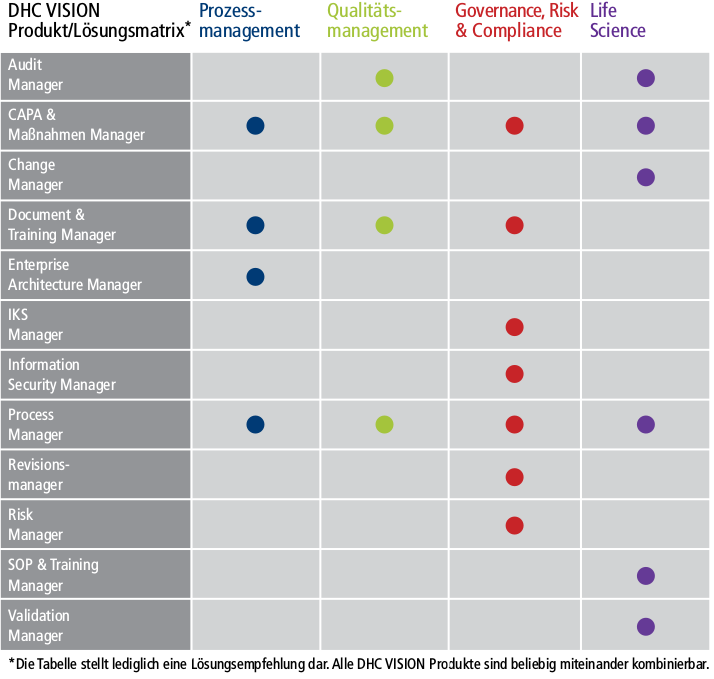
\includegraphics[scale=0.5]{images/dhc.png} 
\caption{DHC VISION Produkt/Lösungmatrix wie sie auf der Produktwebseite\cite{dhc} zu finden ist.}
\end{figure}

Die Features des Information Security Managers werden auf der Webseite\cite{dhc} wie folgt auszugsweise beschrieben:

\textbf{ISMS Management allgemein}
\begin{itemize}
\itemsep0em
\item IT-Strukturanalyse nach dem Standard des Bundesamts für Sicherheit in der Informationstechnologie (BSI) mit all ihren Komponenten und grafische Visualisierung
\item Schutzbedarfsfeststellung inkl. Beschreibung der Unternehmens-Assets mit Bedrohungen, Schwachstellen und Risiken, z.B. auch auf Basis von Katalogen, wie den BSI-Bausteinen
\item BSI-bestätigte Software zur Vorgehensweise gemäß IT-Grundschutz
\end{itemize}

\textbf{ISMS Maßnahmen-Management}
\begin{itemize}
\itemsep0em
\item Definition, Durchführung, Dokumentation und Nachverfolgung von Maßnahmen
\item Erinnerung an Termine bzgl. eingeleiteter Maßnahmen inkl. Eskalationsmechanismen
\item Prüfung der Wirksamkeit der eingeleiteten Maßnahmen
\item Konfigurierbare Workflows zur Abarbeitung und zum formalen Abschluss (inkl. elektronischer Signaturen) der Maßnahmen
\end{itemize}

\textbf{ISMS Dokumentation}
\begin{itemize}
\itemsep0em
\item Erstellung von Sicherheitskonzepten und anderen Dokumenten auf Basis hinterlegter evtl. auch gruppenspezifischer Vorlagen
\item Integration in die Geschäftsprozesse
\item Erfassung von Sicherheitsvorfällen zu Assets
\item Verlinkung zwischen den Dokumenten und zu anderen Objekten (wie Produkten) zur besseren Auffindbarkeit
\end{itemize}

\textbf{Weitere Funktionen}
\begin{itemize}
\itemsep0em
\item Übersichtliche System-Cockpits und rollenspezifische Zugänge
\item Intelligentes Mandantenkonzept für internationale Unternehmen (mehrere Standorte,  verschiedene Sprachen)
\item Nutzer-Akzeptanz durch Integration der Microsoft-Produkte (Visio, Word, Excel, Project)
\item Umfangreiches Berichtswesen sowie Reporting
\item Granulares Berechtigungs- und Zugriffskonzept auf alle Informationen
\end{itemize}

Es wurde angeboten einen Testserver aufzusetzen, dies hätte jedoch zu lange gedauert und ein zweitägiges Seminar zur Einführung erfordert. Ein Webinar zur Demonstration der Software wurde organisiert. Dieses kam allerdings aufgrund von Terminunstimmigkeiten nicht zustande. Daher konnte das Tool nicht bewertet werden. Da der Support sehr zuvorkommend ist und die angegebenen Features gut zu unseren Kriterien passen, wird eine weitere Beschäftigung mit dem Tool empfohlen.
\subsection{SAVe - Security Audit and Verification}
\begin{table}[h!tb]
	%\centering
	\begin{tabular}{|p{0.5\textwidth}|p{0.5\textwidth}|}
		\hline 
		Kriterium & Bewertung\\ 
		\hline 
		\textbf{GUI}& \\
		\hline
		Wizard & 6\\
		\hline 
		Infrastrukturdarstellung & 0 \\
		\hline 
		Netzpläne & 0 \\
		\hline 
		Prozessflüsse & 0 \\
		\hline 
		Schnelles Einpflegen von Änderungen & 10 \\
		\hline
		\textbf{Objektrelationen} & \\
		\hline 
		Doppelseitige Verlinkungen & 5 \\
		\hline 
		Vererbung & 3 \\
		\hline 
		Gruppierungen & 3 \\
		\hline 
		\textbf{Funktionalität} &\\
		\hline 
		Aktuelle BSI-Standards & 2 \\
		\hline  
		Erweiterbarkeit der Klassifizierungen & 2 \\
		\hline 
		Individuelle Beschreibungen & 8 \\
		\hline 
		Sicherheitsverstöße markieren & 2 \\
		\hline
		Bewertung des Sicherheitsstatus & 0 \\
		\hline
		Export von Berichten & 2 \\
		\hline
		BSI-Toolimport & 0 \\
		\hline
		Sicherheit des Tools an sich & 7 \\
		\hline
		Risikobewertung & 0 \\
		\hline
		\textbf{System}&  \\
		\hline
		Verteiltes Arbeiten & 1 \\
		\hline
		Rechtevergabe & 10 \\
		\hline
		Kosten & 4 \\
		\hline
		Support & 3 \\
		\hline
		Zertifizierung & 0 \\
		\hline
		Dokumentation & 2 \\
		\hline
		Marktpräsenz & 4 \\
		\hline
		Spezielle Zielgruppe & 1 \\
		\hline
		Pflege/Weiterentwicklung & 7 \\
		\hline
		\multicolumn{2}{c}{}\\
		\hline
		\textbf{Gesamt} & \\
		\hline
		Hochschuleinsatz & 33\%\\
		\hline
		Lehre & 31\%\\
		\hline
	\end{tabular} 
	\caption{Berwertung: SAVe}
	\label{tab:BerwertungSave}
\end{table}
SAVe\footnote{\url{http://www.infodas.de/DE/Produkte/SAVe}} ist ein weiteres Tool, welches vom BSI als Ersatz für das Grunschutztool empfohlen wird. Im Vergleich zum Grundschutztool kostet SAVe für 10 Lizenzen 7780,00 Euro plus 1167,00 Euro pro Jahr. Voraussetzung für das Programm ist Microsoft Access, welches zusätzlich gekauft werden muss. Für 10 Lizenzen der aktuellen Version von Microsoft Access sind 1350,00 Euro fällig. Damit wären für das erste Jahr 10297,00 Euro zu zahlen.\\
Für die Evaluation des Tools stand eine kostenlose 30-Tage Testversion zur Verfügung, die laut Hersteller keine Einschränkungen besitzt. Möchte man die kostenlose Testversion vom Hersteller bestellen, so kostet dies 49,99 Euro.\\
\\
Die Bewertung aus Tabelle \ref{tab:BerwertungSave} wird im Folgenden näher erläutert:\\
Eine Dokumentation ist sehr wichtig nicht nur für den Einsatz in der Lehre, sondern auch für den Einsatz in einer Firma. Es war jedoch nicht möglich diese Aufzurufen, obwohl sie im Programm enthalten ist. In diesem Fall kann man entweder auf Kulanz des Herstellers hoffen oder man benötigt einen gültigen Wartungsvertrag, da nur dieser die Reparatur defekter Programmversionen umfasst. Die fehlende Dokumentation erschwert auch die Bewertung, da es auch möglich ist, dass manche Funktionalität mit einer Dokumentation aufzufinden gewesen wäre.\\
Bei den BSI-Standards verhält es sich ähnlich. Sie sollen zwar im Programm enthalten sein, jedoch ist ein Anzeigen nicht möglich, was die Funktionalität der Software stark eingrenzt.\\
\\
Ein Wizard ist zwar vorhanden bietet jedoch keine Erklärungen, die bei der Verwendung des Programms helfen. Dennoch ist es hilfreich, um die einzelnen Schritte in der richtigen Reihenfolge durchzuführen. Grafische Darstellung wie Infrastruktur, Netzpläne und Prozessflüsse fehlen komplett in der Anwendung. Dies liegt mit Sicherheit daran, das SAVe lediglich ein Access Add-In ist. Schnelles Einpflegen von Änderungen ist mit dem Programm sehr leicht durchführbar.\\
\\
Doppelseitige Verlinkungen sind in der Anwendung zwar enthalten, jedoch gibt es keine Möglichkeit einer einseitigen Verlinkung. Eine Vererbung ist generell enthalten, jedoch gibt es auch hier nicht die Möglichkeit einer Auswahl, sondern die Bewertung wird immer vererbt. Die Gruppierung im Programm ist folgendermaßen gestaltet: Informationen, Anwendungen, IT-Systeme, Räume und Kommunikationsverbindungen.\\
\\
Eine Erweiterung der Klassifizierung ist teilweise möglich. Es können neue angelegt werden, jedoch gibt es keine Möglichkeit einer Spezifizierung dieser. Individuelle Beschreibungen sind an jeder Stelle möglich, jedoch fehlt der Zwang eine Beschreibung in speziellen Fällen eintragen zu müssen, wie es im Grundschutztool vorhanden ist. Sicherheitsverstöße werden an keiner Stelle prominent angezeigt, sondern müssen selbst per Hand herausgesucht werden. Eine Detaillierte Bewertung des Sicherheitsstatus war in keiner Ansicht zu finden. Ein Export von Berichten ist zwar möglich, jedoch nur in Form einer CSV-Datei oder einer Excel-Tabelle, die in diesem Fall komplett in Englisch ist, obwohl das Programm komplett auf Deutsch ist. Ein Import vom Grundschutztool soll zwar laut Internetseite möglich sein, jedoch ist eine Option dafür an keiner Stelle zu finden. Die Datenbank kann durch ein Passwort abgesichert werden, jedoch kann jeder, der das Passwort hat, sich die Rolle selbst aussuchen, wodurch eine Rollenvergabe nicht sinnvoll möglich ist. Eine Risikobewertung kann selbständig durchgeführt werden und ist nicht weiter unterstützt.\\
\\
Ein verteiltes Arbeiten wird vom Programm an sich nicht unterstützt, jedoch ist es über Umwege möglich. Eine Rechtevergabe ist möglich, jedoch muss jeder Anwender selbständig darauf achten, dass er die richtige Rolle verwendet. Eine Zertifizierung aufgrund des Programms ist generell nicht möglich. Das Tool wird vom BSI empfohlen, wodurch die Marktpräsenz relativ gut zu bewerten ist. Das Tool ist für alle Nutzergruppen konzipiert. Es möglich eine oder mehrere Consulting-Editionen zu erwerben, dies kostet jedoch pro Lizenz 100 Euro extra. Auch der Kauf einer Version für die Bundeswehr ist auf Anfrage mit Aufpreis möglich. Die aktuelle Version ist vom März 2014. Die vorhergehende Version ist vom September 2012, wodurch auf eine gute Weiterentwicklung zu schließen ist.\\
\\
Bedauerlich jedoch ist, das die Internetseite nicht aktuell ist, was einem einen schlechten Eindruck vermittelt. Insgesamt ist die Software nicht zu empfehlen.
\subsection{Adamant}
Adamant ist ein kostenloses Open-Source Tool zum gemeinsamen Management von Sicherheitsanforderungen. Dazu unterstützt es die Modellierung von Requirements auf Grundlage von zum Beispiel dem BSI-Grundschutzkatalog.\cite{adamant}\\ 
Zum Testen stand nur eine Live-Demo der Software zur Verfügung, so dass das Beispiel der Hochschule nicht nach modelliert werden konnte. Die Bewertung gründet sich damit auf den in der Live-Demo beispielhaft zur Verfügung gestellten Daten.\\

\begin{table}[h!bt]
	%\centering
	\begin{tabular}{|p{0.5\textwidth}|p{0.5\textwidth}|}
		\hline 
		Kriterium & Bewertung\\ 
		\hline 
		\textbf{GUI}& \\
		\hline
		Wizard & 0\\
		\hline 
		Infrastrukturdarstellung & 8 \\
		\hline 
		Netzpläne & 0 \\
		\hline 
		Prozessflüsse & 0 \\
		\hline 
		Schnelles Einpflegen von Änderungen & 8 \\
		\hline
		\textbf{Objektrelationen} & \\
		\hline 
		Doppelseitige Verlinkungen & 8 \\
		\hline 
		Vererbung & 0 \\
		\hline 
		Gruppierungen & 0 \\
		\hline 
		\textbf{Funktionalität} &\\
		\hline 
		Aktuelle BSI-Standards & 5 \\
		\hline  
		Erweiterbarkeit der Klassifizierungen & 7 \\
		\hline 
		Individuelle Beschreibungen & 8 \\
		\hline 
		Sicherheitsverstöße markieren & 8 \\
		\hline
		Bewertung des Sicherheitsstatus & 4 \\
		\hline
		Export von Berichten & 6 \\
		\hline
		BSI-Toolimport & 0 \\
		\hline
		Sicherheit des Tools an sich & 0 \\
		\hline
		Risikobewertung & 0 \\
		\hline
		\textbf{System}&  \\
		\hline
		Verteiltes Arbeiten & 5 \\
		\hline
		Rechtevergabe & 0 \\
		\hline
		Kosten & 7 \\
		\hline
		Support & 2 \\
		\hline
		Zertifizierung & 0 \\
		\hline
		Dokumentation & 0 \\
		\hline
		Marktpräsenz & 0 \\
		\hline
		Spezielle Zielgruppe & 0 \\
		\hline
		Pflege/Weiterentwicklung & 8 \\
		\hline
		\multicolumn{2}{c}{}\\
		\hline
		\textbf{Gesamt} & \\
		\hline
		Hochschuleinsatz & 35\%\\
		\hline
		Lehre & rund 43\%\\
		\hline
	\end{tabular} 
	\caption{Bewertung: Adamant}
	\label{tab:BewertungAdamant}
\end{table}
Für die Kriterien Wizard, Netzpläne und Prozessflüsse unter dem Punkt GUI wurden jeweils 0 Punkte vergeben, da das Tool nicht über Wizards zur Projekterstellung oder Erstellung zum Beispiel eines zu schützenden Wertes oder Risikos verfügt beziehungsweise keine Netzpläne oder Prozessflüsse modelliert und dargestellt werden können. Die Infrastrukturdarstellung erhielt 8 Punkte, da eine gute hierarchisch organisierte Übersicht über die angelegten Assets abrufbar ist. Punktabzug gab es hier nur weil die Navigation in dieser Hierarchie etwas umständlich ist. Auch erhielt das Kriterium der schnellen Einarbeitung von Änderungen ein Bewertung von 8, da es über die Metadaten (Meta Data) recht einfach ist alle relevante Objekte wie die zu schützenden Werte (Assets), die Risiken (Risks), die Quellen (Soucres) die für ein Requirement hinterlegt werden können und die zuständigen Stellen (Stakeholder) zu editieren oder anzulegen.\\
\begin{figure}[h!bp]
\label{fig:admantHierarchie}
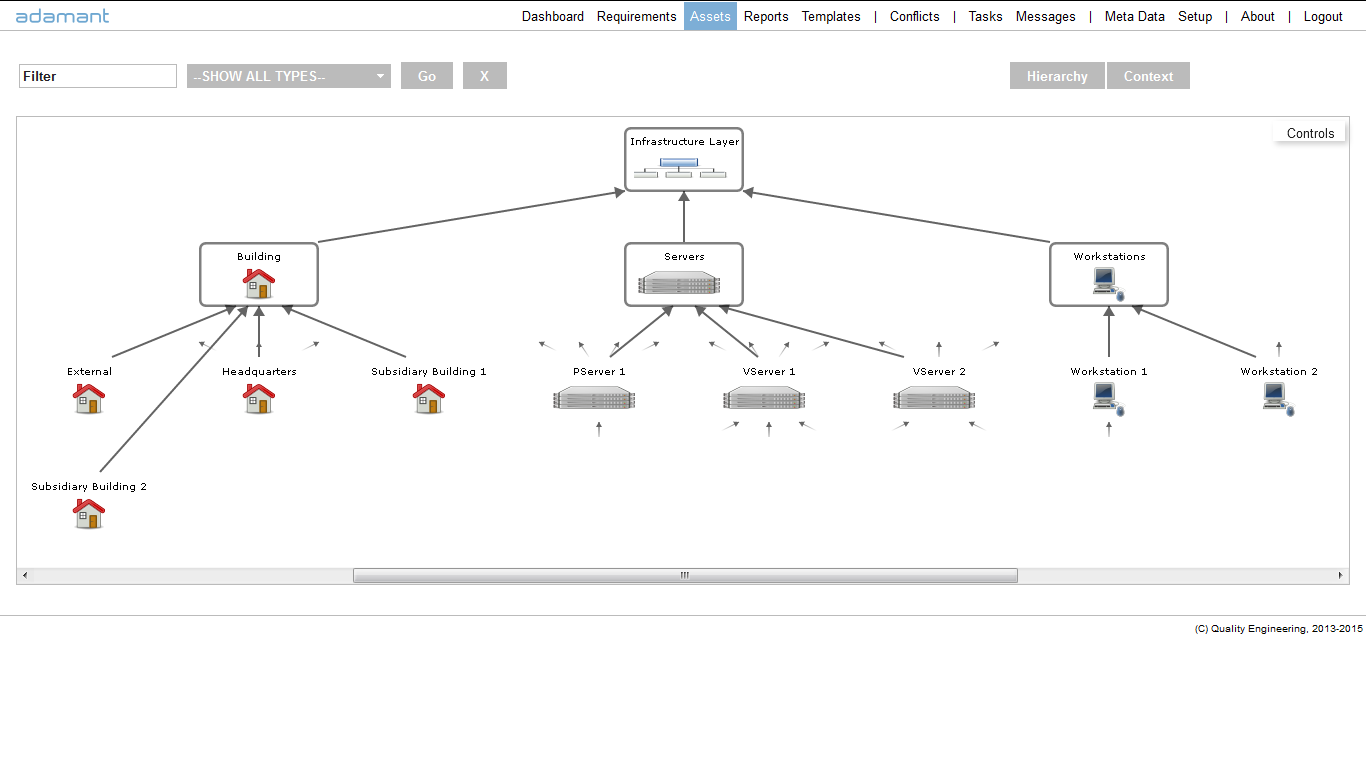
\includegraphics[scale=0.40]{images/adamant_hierarchie.png} 
\caption{Hierarchische Darstellung der Infrastruktur mit Adamant}
\end{figure}\\
Bei den Objektrelationen erhielt die doppelseitigen Verlinkungen 8 Punkte, da diese über die Metadaten (Meta Data) einfach zwischen den Assets hinterlegt werden können. Punktabzug gab es hier da nicht zu erkennen war, dass sich diese Verlinkungen auf die Sicherheitsbewertung ausgewirkt haben. Hingegen wurden die Vererbung und die Gruppierung mit 0 Punkten bewertet, da diese nicht möglich sind.\\
Unter den Funktionalitäten des Tools wurde die Erweiterbarkeit der Klassifizierungen mit 7 Punkten bewertet, weil sowohl die Erfüllungs- als auch die Revalidierungsmodelle sowie die Prioritäten um eigene Klassen erweiterte werden können. Die individuellen Beschreibungen erhielten 8 Punkte, da sie für alle Objekte hinterlegt werden können, sowohl für einzelne Assets oder Risiken als auch für die Report und die Requirements. Der Export von Berichten wurde mit 6 Punkten bewertet, weil es zwar möglich ist Reports zu erstellen und auch eigene zu definieren, diese aber recht wenig aussagekräftig sind. Für die aktuellen BSI-Standards gab es 5 Punkte, da zum Zeitpunkt der Analyse die Standards von 2013 als Grundlage dienten, aber keine Möglichkeit erkenntlich war neue Standards einzupflegen, wie zum Beispiel eine Update-Funktion. Es kann aber auch möglich sein das eine derartige Funktion in der Live-Demo nur deaktiviert ist und somit nicht angezeigt wird. Der GS-Tool Import erhielt eine Bewertung von 0 Punkten, da keine Funktion zum Importieren von Modellen aus dem Grundschutz-Tool des BSI vorhanden ist. Die Markierung von Sicherheitsverstößen wurde mit 8 Punkten bewertet und die Bewertung des Sicherheitsstatus mit 4 Punkten, da das Programm nur jene der selbsterstellen Requirements markiert, die nicht erfüllt sind oder revalidiert werden müssen. Die Sicherheit des Tools an sich erhielt eine Bewertung von 0 Punkten, da es keine Angaben über eine Verschlüsselung der gespeicherten Daten oder eine andere Schutzmaßnahme für die Daten gibt. Die zusätzliche Risikobewertung wurde mit 0 Punkten bewertet, weil das Programm eine solche nicht unterstützt.\\
\begin{figure}[h!bp]
\label{fig:admantReports}
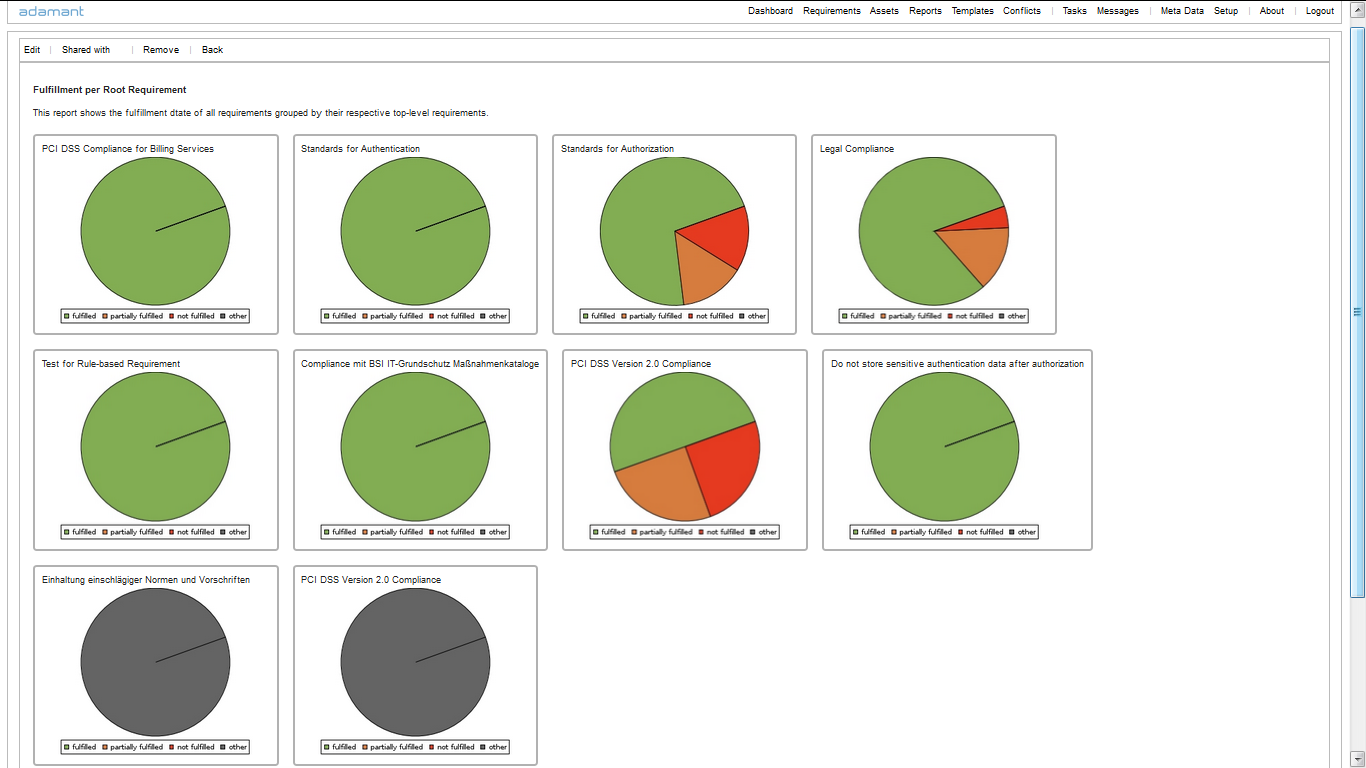
\includegraphics[scale=0.40]{images/adamant_reports.png} 
\caption{Mit Adamant erstellter Erfüllungsbericht für Sicherheitsanforderungen}
\end{figure}
Unter dem Punkt System wurde das verteilte Arbeiten mit einer Bewertung von  5 versehen, da es webbasiert ist und für das gemeinsame Entwickeln der Sicherheitsanforderungen konzipiert ist. Punktabzug gab es weil Softwareseitig, in der Live-Demo, keine Rechtevergabe möglich war. Daher auch die 0 Punkte für das Kriterium Rechtevergabe. Eine Zertifizierung durch Einsatz dieses Programms ist nicht möglich, daher gab es auch hierfür 0 Punkte. Auch für Marktpräsenz und Nutzerkreis gab es 0 Punkte, da keine Referenzen gefunden werden konnten, dass dieses Programm produktiv im Einsatz ist und kein bestimmter Nutzerkreis aus zu machen ist. Auch die Dokumentation erhielt 0 Punkte, weil keine gefunden werden konnte. Der herrunterladbaren Source-Code soll auch eine Dokumentation beiliegen, was leider nicht überprüft werden konnte, da der Versuch des Download immer mit einer Fehlermeldung endete. Für die Kosten wurden 7 Punkte vergeben, weil es sich um ein kostenloses Open-Soucre Tool handelt, welches noch weiterentwickelt wird. Deshalb erhielt auch Pflege/Weiterentwicklung 8 Punkte.\\

\subsection{GSTool}

Mit dem GSTOOL Programm vom BSI (Bundesamt für Sicherheit in der Informationstechnik) kann man entsprechende Sicherheitskonzepte
nach dem Verfahren des IT-Grundschutzes modellieren.
1994 wurde das IT-Grundschutzhandbuch veröffentlicht und nach 4 Jahren wurde das GSTOOL herausgegeben.
Die Verwendung von GSTOOL ist umsonst.

\subsubsection{Bewertung}

GUI des GSTOOLs ist übersichtlich und sehr nutzerfreundlich. Man kann sehr leicht die Komponenten finden und bedienen. Trotzdem gibt es keine Möglichkeit, die Netzpläne und Prozessflüsse darzustellen. Man kann auch nicht nur die doppelseitige Verlinkungen erstellen sondern auch die individuelle Beschreibungen. Was den Export von Berichten betrifft, besteht auch keine Möglichkeit.     

Wenn es um die Pflege und Weiterentwicklung geht, wird der Support nur bis Ende 2016 unterstützt. Deshalb steht in der Bewertung 0. 

Beim Support wurde nicht schnell auf die Emails geantwortet. Der Grund liegt vielleicht an der Weihnachtzeit.  



Die GSTOOL-Lizenzen sind frei für unmittelbare Bundes-, Landes- und Kommunalverwaltungen Deutschlands.
Einrichtungen der Forschung und Lehre bekommen einen Rabatt auf die unten genannten Preise.
Für alle anderen Besteller gilt folgende Preistabelle (Abbildung~\ref{fig:GSToolschema}).
Die gesamten Kosten, die die Tabelle darstellt, sind hoch im Vergleich mit anderen Lösungen. Daher gibt es 5 in der Tabelle, es stellt somit ebenfalls den Referenzwert dar.  


\begin{figure}[htbp]
	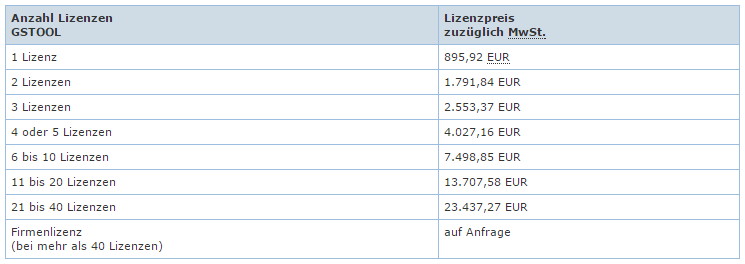
\includegraphics[scale=0.6]{images/gstoolpreis}
	\caption{Preise des GSTools}
	\label{fig:GSToolschema}
\end{figure}

Der Unterschied zwischen Hochschuleinsatz und Lehre ist nur $0.9\%$. Der Hochschuleinsatz hat $67.2\%$ und der Lehreinsatz $68.1\%$. Damit ist dieses Programm in fast gleichem Maß für beide Bereiche geeignet.

\subsubsection{Darstellung des Fallbeispiels}

Mithilfe des GSTOOls wurde das Beispiel der Hochschule modelliert. Das Beispiel ist in vollem Maß darstellbar, jedoch präsentiert das Programm den Baum nicht so ganz korrekt.  

\begin{figure}[htbp]
	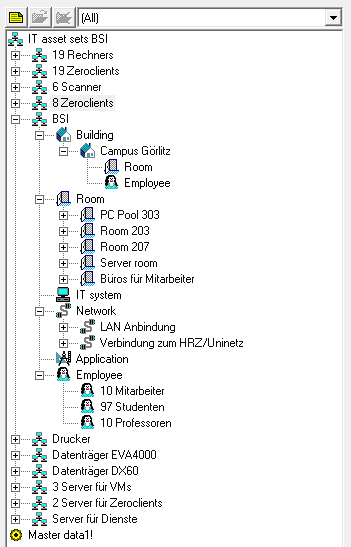
\includegraphics[scale=0.5]{images/gstooltree}
	\caption{Beispiel der Hochschule in GSTool}
	\label{fig:GSTooltree}
\end{figure}  


\begin{table}[h!bt]
%\centering
\begin{tabular}{|p{0.5\textwidth}|p{0.5\textwidth}|}
\hline 
Kriterium & Bewertung\\ 
\hline 
\textbf{GUI}& \\
\hline
Wizard & 7\\
\hline 
Infrastrukturdarstellung & 10 \\
\hline 
Netzpläne & 0 \\
\hline 
Prozessflüsse & 0 \\
\hline 
Schnelles Einpflegen von Änderungen & 10 \\
\hline
\textbf{Objektrelationen} & \\
\hline 
Doppelseitige Verlinkungen & 0 \\
\hline 
Vererbung & 10 \\
\hline 
Gruppierungen & 8 \\
\hline 
\textbf{Funktionalität} &\\
\hline 
Aktuelle BSI-Standards & 10 \\
\hline  
Erweiterbarkeit der Klassifizierungen & 10 \\
\hline 
Individuelle Beschreibungen & 0 \\
\hline 
Sicherheitsverstöße markieren & 10 \\
\hline
Bewertung des Sicherheitsstatus & 10 \\
\hline
Export von Berichten & 0 \\
\hline
BSI-Toolimport & 10 \\
\hline
Sicherheit des Tools an sich & 10 \\
\hline
Risikobewertung & 10 \\
\hline
\textbf{System}&  \\
\hline
Verteiltes Arbeiten & 10 \\
\hline
Rechtevergabe & 10 \\
\hline
Kosten & 5 \\
\hline
Support & 5 \\
\hline
Zertifizierung & 10 \\
\hline
Dokumentation & 7 \\
\hline
Marktpräsenz & 10 \\
\hline
Spezielle Zielgruppe & 8 \\
\hline
Pflege/Weiterentwicklung & 0 \\
\hline
\multicolumn{2}{c}{}\\
\hline
\textbf{Gesamt} & 190\\
\hline
Hochschuleinsatz & $67,2\%$\\
\hline
Lehre & $68,1\%$\\
\hline
\end{tabular} 
\caption{Bewertung: GSTool}
\label{tab:BewertungGSTool}
\end{table}

\subsection{I-doit}

Bei I-doit handelt es sich um eine von \textit{synetics} entwickelte webbasierte Software, die zur Abbildung komplexer IT-Infrastrukturen dient.
Dabei stehen dem Anwender verschiedene Komponenten zur Verfügung. 
Die aktuelle Version ist dabei 1.4.8 (31.Oktober 2014). 

Die zentrale Komponente, die sogenannte \textit{Configuration Management Database (CMDB)} dient dabei dem Nutzer zum anlegen verschiedener Objekte, wie z.B. Workflows, IT-Systeme, Kontakte und Services.
Weitere Komponenten wie Import oder Export sind ebenfalls enthalten.
Ein Reportmanager erleichtert den Umgang mit dokumentierten Daten. 
Durch die Plattformunabhängigkeit und die standardisierten Programmiersprachen PHP, MySQL und Javascript wird ein flexibler Einsatz gewährleistet.

I-doit ist in zwei Versionen verfügbar. Zum Einen eine frei verfügbare Open-Source Version und zum Anderen eine kostenpflichtige Pro Version.
Die Unterschiede sowie die verschiedenen Preise in Hinblick auf die Pro Version sind in Abbildung~\ref{fig:idoitvergleich} und Abbildung~\ref{fig:idoitpreis} einsehbar.

\begin{figure}[htbp]
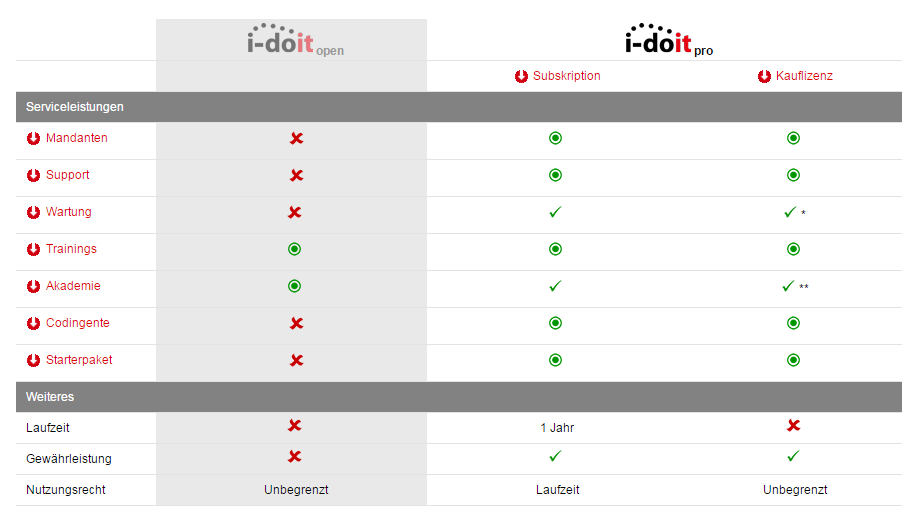
\includegraphics[width=\textwidth]{images/idoitvergleich}
\caption{Vergleich der Versionen von I-doit im Vergleich}
\label{fig:idoitvergleich}
\end{figure}

\begin{figure}[htbp]
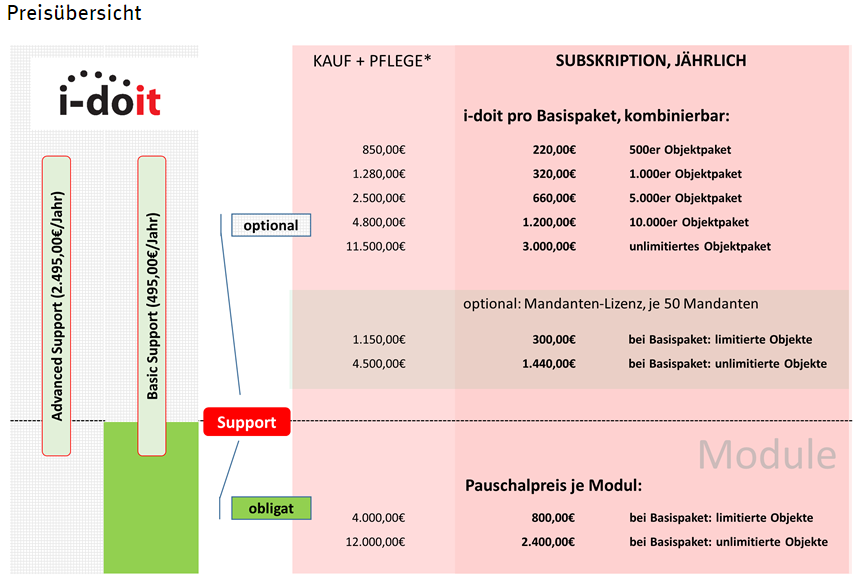
\includegraphics[width=\textwidth]{images/idoitpreis}
\caption{Preise der Versionen von I-doit im Vergleich}
\label{fig:idoitpreis}
\end{figure}

Durch ein Rechtesystem sind administrative Regelungen problemlos möglich, da verschiedene Rollen vergeben werden können.
Das bedeutet, Anwender können einer Personengruppe zugeordnet werden, die verschiedene Rechte wie Lese-, Schreib- oder Administrationsrechte beinhalten.

Ein weiteres Feature von I-doit ist die Mandantenfähigkeit, wodurch innerhalb einer I-doit Instanz verschiedene Mandanten komplett voneinander getrennt entworfen werden können.
Bei der Erzeugung von Objekten wird der Anwender durch Templates unterstützt.
So können z.B. verschiedene Rechner vom gleichen Typ mehrfach abgebildet werden, ohne alle einzeln zu erstellen.

Das Reporting von I-doit, welches auf den I-doit Datenbanken basiert, ermöglicht ein automatisiertes Erstellen und Auswerten der eingetragenen Objekte.
In den Reports werden wichtige Eckdaten wie Statistiken zur abgebildeten Infrastruktur zusammengefasst.
Dabei stehen die Formate Text, PDF, CSV und XML zur Verfügung.

Ein wesentlicher Unterschied, den wir ohne eine Testversion der kostenpflichtigen Variante von I-doit feststellen konnten, liegt in der Sprachunterstützung.
Die Open-Source Version ist lediglich in englischer Sprache verfügbar, wohingegen die Pro Version mehrsprachig entwickelt wurde.


\subsubsection{Umsetzung des Fallbeispiels}
Nachfolgend sind in Abbildung~\ref{fig:idoittree} und Abbildung~\ref{fig:idoitschema} die Resultate der Übertragung des Fallbeispiels nach I-doit zu sehen.
Darauf zu sehen ist die Infrastruktur, die durch das Fallbeispiel definiert ist, mit den entsprechenden Objekten und deren Verknüpfungen.
Abbildung~\ref{fig:idoittree} zeigt die Standortansicht, in der die Objekte hinzugefügt und angelegt werden, wohingegen Abbildung~\ref{fig:idoitschema} die CMDB Ansicht darstellt.
Aus Platzgründen konnte die schematische Darstellung von Abbildung~\ref{fig:idoitschema} hier nicht vollständig dargestellt werden.

\begin{figure}[htbp]
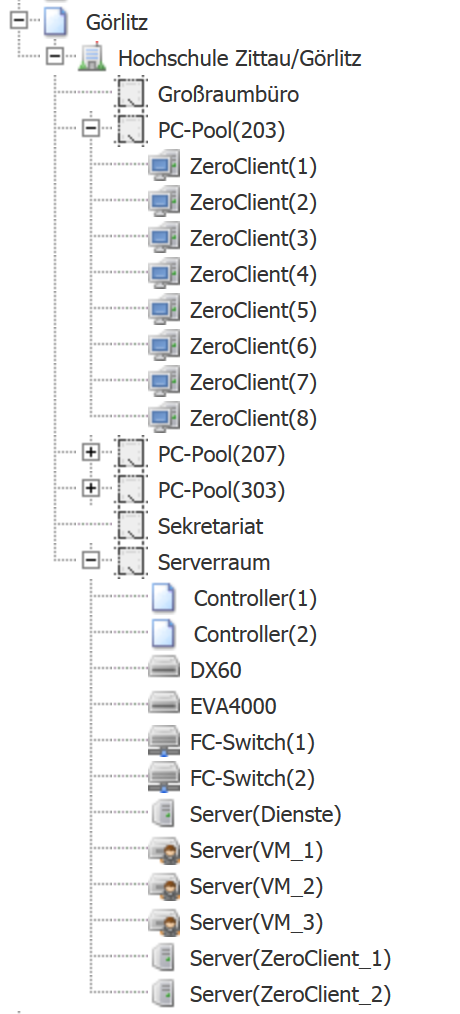
\includegraphics[scale=1]{images/idoittree}
\caption{Baumstruktur in I-doit}
\label{fig:idoittree}
\end{figure}

\begin{figure}[htbp]
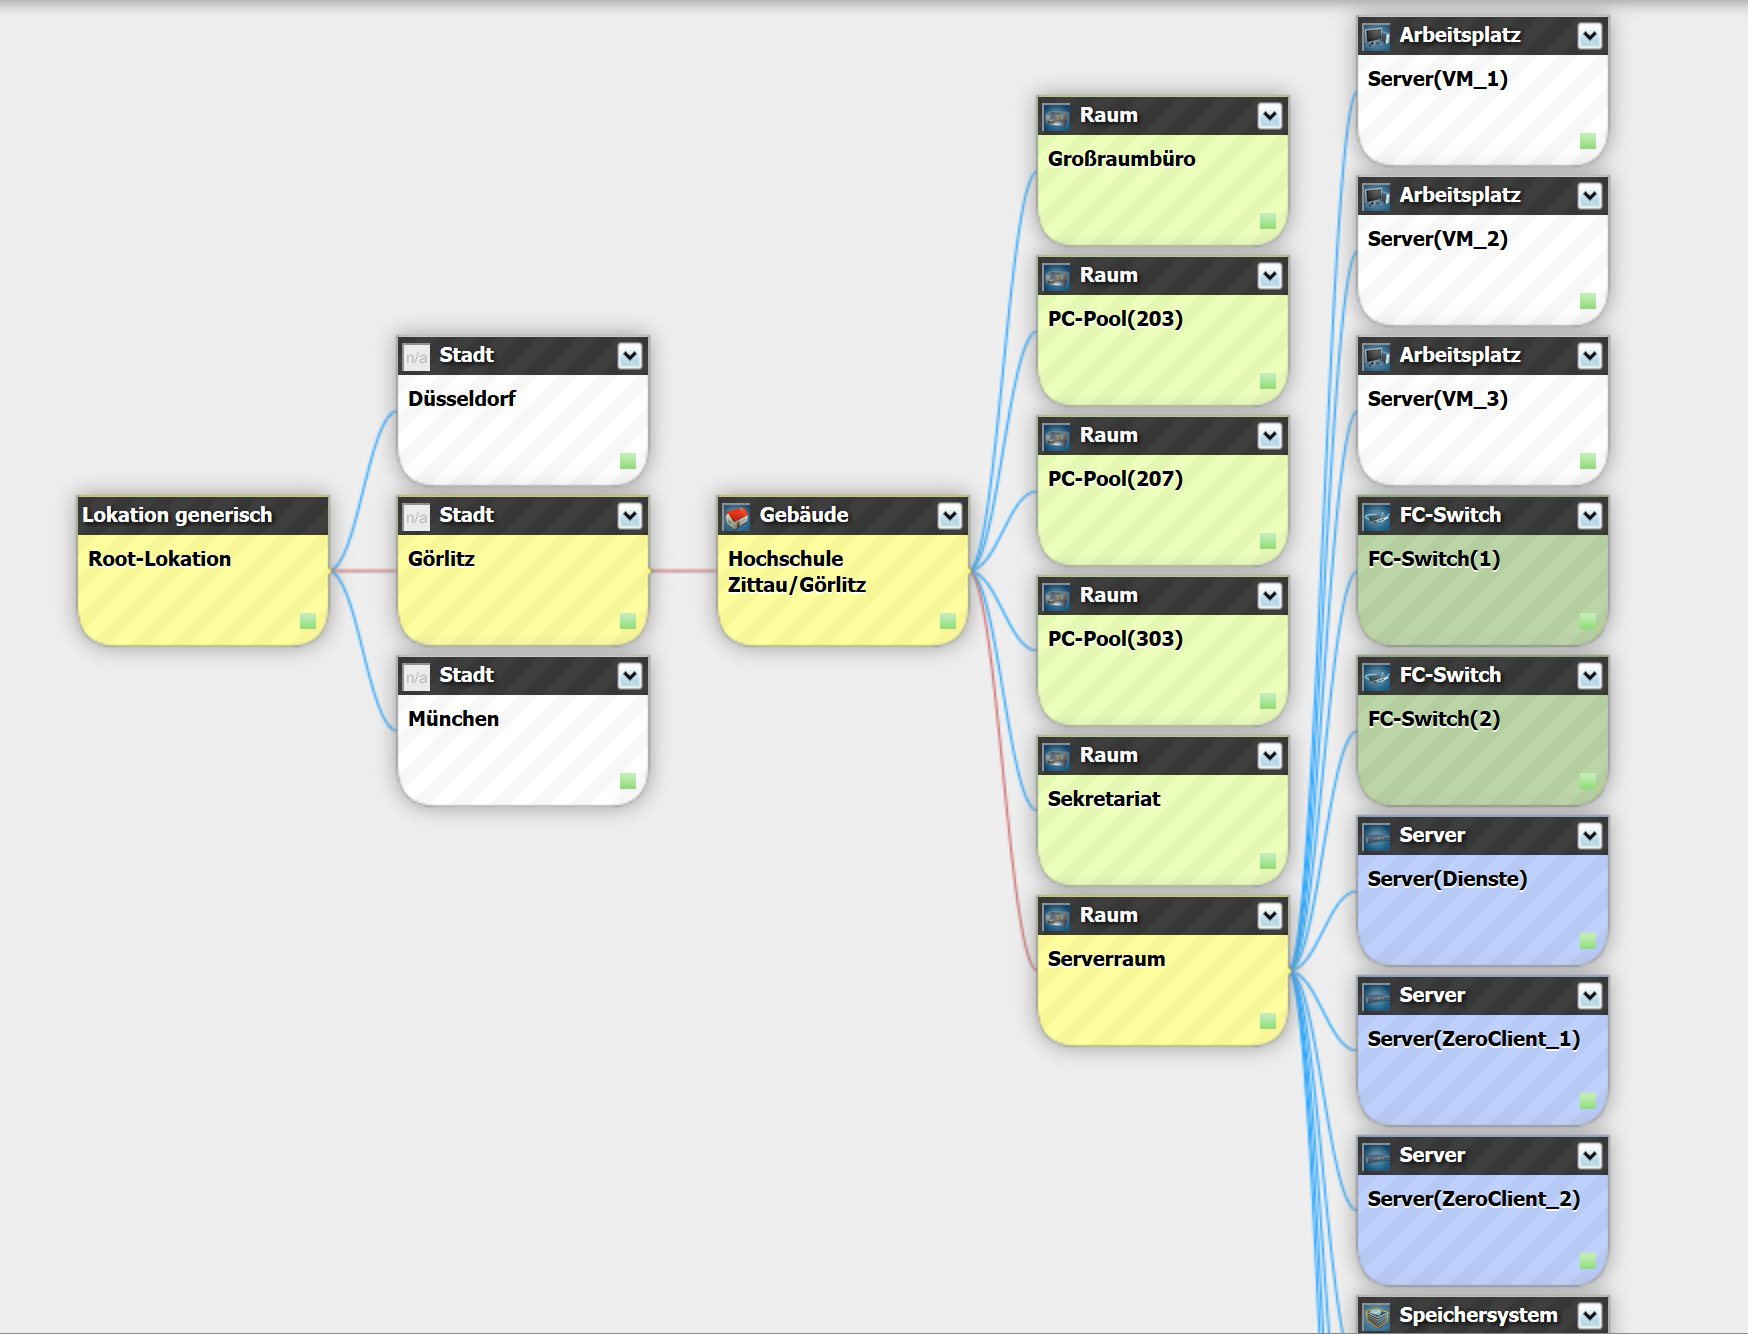
\includegraphics[width=\textwidth]{images/idoitschema}
\caption{Infrastrukturdarstellung in I-doit}
\label{fig:idoitschema}
\end{figure}


\subsubsection{Bewertungsergebnisse}
Tabelle~\ref{tab:BerwertungIdoit} zeigt die Punkteverteilung für das Tool I-doit. 
Die möglichen Bereiche spannen sich von 0 (nicht vorhanden) bis 10 (sehr gut).
Allgemein betrachtet erzielte I-doit eine gute Gesamtbewertung mit 221 von maximal 280 erreichbaren Punkten.
Gemäß der vorher festgelegten Wichtungen eignet sich I-doit damit mit ca. $82,5\%$ für den Gebrauch durch die Hochschule und mit ca. $83,4\%$ für den Gebrauch für die Lehre
an der Hochschule.

Negativ kristallisierten sich Aspekte im Bereich der Vererbung heraus. Hier wurden Werte bezüglich der Integrität, der Authentizität und der Verfügbarkeit nicht an Elternelemente vererbt. Andere Werte, wie der Zustand der Objekte, wurden dagegen weitergegeben.
Ein weiterer negativer Aspekt ist die Funktion zum Export von Berichten. Hierbei ist die Flexibilität für die Erstellung eines Reports nur sehr beschränkt möglich.
Auch die Risikobewertung, welche die aktuelle Situation der Infrastruktur bewerten soll, war nur begrenzt vorhanden. 

Die Usabilty von I-doit wird unterstützt durch zahlreiche Templates. Nichtsdestotrotz ist die Menüführung für die Erstellung und Verknüpfung von Objekten nicht intuitiv und bringt eine längere Einarbeitungszeit mit sich.

\begin{table}[h]
%\centering
\begin{tabular}{|p{0.5\textwidth}|p{0.5\textwidth}|}
\hline
Kriterium & Bewertung\\
\hline
\textbf{GUI}& \\
\hline
Wizard & 5 \\
\hline
Infrastrukturdarstellung & 10 \\
\hline
Netzpläne & 6 \\
\hline
Prozessflüsse & 8 \\
\hline
Schnelles Einpflegen von Änderungen & 7 \\
\hline
\textbf{Objektrelationen} &  \\
\hline
Doppelseitige Verlinkungen & 10 \\
\hline
Vererbung & 4 \\
\hline
Gruppierungen & 10 \\
\hline
\textbf{Funktionalität} &\\
\hline
Aktuelle BSI-Standards & 10 \\
\hline
Erweiterbarkeit der Klassifizierungen & 10 \\
\hline
Individuelle Beschreibungen & 10 \\
\hline
Sicherheitsverstöße markieren & 8 \\
\hline
Bewertung des Sicherheitsstatus & 10 \\
\hline
Export von Berichten & 5 \\
\hline
BSI-Toolimport & 10 \\
\hline
Sicherheit des Tools an sich & 8 \\
\hline
Risikobewertung & 5 \\
\hline
\textbf{System}& \\
\hline
Verteiltes Arbeiten & 10 \\
\hline
Rechtevergabe & 10 \\
\hline
Kosten & 10 \\
\hline
Support & 10 \\
\hline
Zertifizierung & 10 \\
\hline
Dokumentation & 5 \\
\hline
Marktpräsenz & 10 \\
\hline
Spezielle Zielgruppe & 10 \\
\hline
Pflege/Weiterentwicklung & 10 \\
\hline
\multicolumn{2}{c}{}\\
\hline
\textbf{Gesamt} & 221\\
\hline
Hochschuleinsatz & $82,5\%$\\
\hline
Lehre & $83,4\%$\\
\hline
\end{tabular}
\caption{Bewertung: I-doit}
\label{tab:BerwertungIdoit}
\end{table}



\subsection{Audit-Tool 2009}
Beim \textit{Audit-Tool~2009} handelt es sich um ein Produkt der Firma \textit{Secure-IT}.
Auf der Website wird damit geworben, dass sich das Tool für eine grobe Strukturanalyse und eine grobe Modellierung eignet.
Weiterhin wird damit geworben, dass das Tool das aktuelle Sicherheitsniveau anzeigt. Auch sollen die Stärken und Schwächen  der
eigenen IT-Sicherheit angezeigt werden.
Im Abschluss verspricht die Website ebenfalls die Ermittlung der Komponenten für die der 
größte Handlungsbedarf besteht.

Das Tool konnte nicht ausprobiert und bewertet werden, da die Firma keine Testversion bereitgestellt hat.
Es wurden wiederholt Mails an die Firma geschrieben, auf die nicht geantwortet wurde.
Auch der telefonische Kontakt konnte nicht hergestellt werden, da auch bei mehrfachen Versuchen niemand abgenommen hat.
Die letzte Aktualisierung auf der Website fand ende 2012 statt.


\subsection{Verinice}
Verinice ist eine freie und Open-Source-Informationssicherheitsmanagementsystem (ISMS) Anwendung, die bei der Schaffung und Erhaltung von Systemen des Informations- und Sicherheitsmanagements helfen kann.

Verinice wurde von einer deutschen Firma SerNet Service Network GmbH geschrieben und wird gleichzeitig gepflegt.

Verinice steht unter der GNU General Public License (Version 3 oder höher).

Zu den wichtigsten Nutzern gehören kleine und mittlere Unternehmen, einige große Unternehmen und Regierungsbehörden.

In Deutschland wird Verinice als ISMS Tool vom Verband der Automobilindustrie empfohlen
für ihre Mitglieder wie Volkswagen, Daimler AG, Fiat und andere großen Herstellern.
VDA fördert auch Verinice Entwicklung seit Release 1.2.

Verinice unterstützt die Betriebssysteme Windows, Linux und OS X.

\begin{figure}[htbp]
	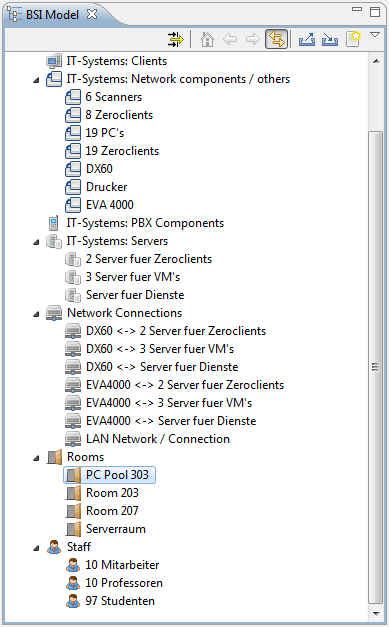
\includegraphics[scale=0.5]{images/verinicestruktur}
	\caption{Infrastrukturdarstellung in Verinice}
	\label{fig:veriniceStruktur}
\end{figure}


\begin{table}[h]
%\centering
\begin{tabular}{|p{0.5\textwidth}|p{0.5\textwidth}|}
\hline 
Kriterium & Bewertung\\ 
\hline 
\textbf{GUI}& \\
\hline
Wizard & 5\\
\hline 
Infrastrukturdarstellung & 7 \\
\hline 
Netzpläne & 0 \\
\hline 
Prozessflüsse & 0 \\
\hline 
Schnelles Einpflegen von Änderungen & 10 \\
\hline
\textbf{Objektrelationen} & \\
\hline 
Doppelseitige Verlinkungen & 10 \\
\hline 
Vererbung & 0 \\
\hline 
Gruppierungen & 10 \\
\hline 
\textbf{Funktionalität} &\\
\hline 
Aktuelle BSI-Standards & 10 \\
\hline  
Erweiterbarkeit der Klassifizierungen & 10 \\
\hline 
Individuelle Beschreibungen & 10 \\
\hline 
Sicherheitsverstöße markieren & 5 \\
\hline
Bewertung des Sicherheitsstatus & 5 \\
\hline
Export von Berichten & 10 \\
\hline
BSI-Toolimport & 10 \\
\hline
Sicherheit des Tools an sich & 8 \\
\hline
Risikobewertung & 5 \\
\hline
\textbf{System}&  \\
\hline
Verteiltes Arbeiten & 10 \\
\hline
Rechtevergabe & 10 \\
\hline
Kosten & 9 \\
\hline
Support & 10 \\
\hline
Zertifizierung & 10 \\
\hline
Dokumentation & 5 \\
\hline
Marktpräsenz & 10 \\
\hline
Spezielle Zielgruppe & 5 \\
\hline
Pflege/Weiterentwicklung & 6 \\
\hline
\multicolumn{2}{c}{}\\
\hline
\textbf{Gesamt} & 190\\
\hline
Hochschuleinsatz & $71,8\%$\\
\hline
Lehre & $64,0\%$\\
\hline
\end{tabular} 
\caption{Bewertung: Verinice}
\label{tab:BerwertungVerinice}
\end{table}








\include{crisam}

\section{Fazit}
Aufgabe war es, einen Ersatz für das derzeit im Einsatz befindliche BSI-GS-Tool zu finden, sowohl für den Einsatz in der Lehre als auch zur Realisierung der IT-Sicherheit an der Hochschule. Untersucht wurden dazu die vom BSI empfohlenen Programme. Die Ergebnisse dieser Untersuchung sind Tabelle~ref{programmvergleich} zu entnehmen.

Als erstes ist hervorstechend, dass einige der empfohlenen Programme nicht mehr gepflegt werden und somit für eine Nutzung in beiden Bereichen ausscheiden. Auch das \textit{BSI-GS-Tool}, welches als Vergleich dient, hat mit den von uns aufgestellten Kriterien nur ca. 70\% der maximalen Punktzahl erreicht. Die höchste Punktzahl, knapp vor \textit{opus i}, erreicht \textit{I-doit} mit 83\% und ist somit unsere Empfehlung als Ersatz für das BSI-GS-Tool. Trotzdem hat es seine Unzulänglichkeiten in einige Bereichen. Abschließend ist zu erwähnen, dass auch wenn nicht alle Programme gute Gesamtwertungen erreicht haben, können sie für machen Ansprüche trotzdem genügen, was im Einzelfall zu prüfen ist. Denn wie eingangs geschrieben zählt die Umsetzung im Unternehmen, dazu ist mit gewissen Abstrichen jedes der testbaren Programme zumindest fähig.
\begin{table}[h!tb]
	%\centering
	\begin{tabular}{|p{0.5\textwidth}|p{0.2\textwidth}|p{0.2\textwidth}|}
		\hline 
		\textbf{Programm} & \textbf{Hochschule} & \textbf{Lehre}\\ 
		\hline
		Sidoc & 52\% & 55\% \\
		\hline 
		Doc SetMinder & \multicolumn{2}{c|}{keine Testversion; zu hohe Einarbeitung}\\
		\hline 
		HiScout & \multicolumn{2}{c|}{Angebot, aber keine freie Testversion} \\
		\hline 
		GRC Suite iRIS & \multicolumn{2}{c|}{keine Testversion; organisatorisch nicht machbar}\\
		\hline 
		opus i & 77\% & 80\% \\
		\hline
		INDART Professional & \multicolumn{2}{c|}{keine funktionierende Testversion} \\
		\hline 
		DHC VISION & \multicolumn{2}{c|}{organisatorisch nicht machbar} \\
		\hline 
		SAVe - Security Audit and Verification & 33\% & 31\% \\
		\hline 
		Adamant & 35\% & 43\%\\
		\hline 
		GS-Tool & 67\% & 68\% \\
		\hline  
		I-doit & 83\% & 83\% \\
		\hline
		Audit-Tool 2009 & \multicolumn{2}{c|}{keine Testversion} \\
		\hline
		Verinice & 72\% & 64\% \\
		\hline
		Crisam & 71\% & 70\% \\
		\hline
	\end{tabular} 
	\caption{Vergleich der getesteten Programme}
	\label{tab:programmvergleich}
\end{table}
%section
\section{Anhang}
\begin{appendix}

\section{opus i}
\begin{figure}[H]
\label{opusiimage}
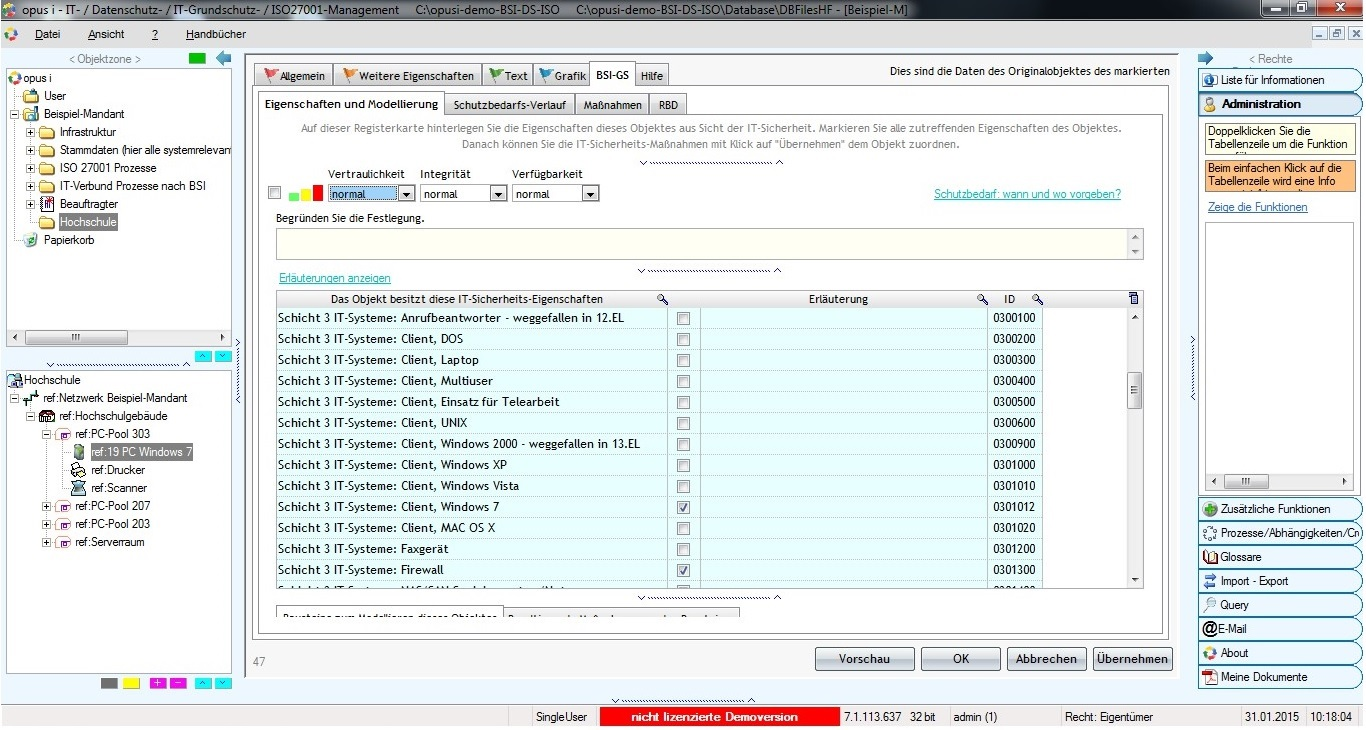
\includegraphics[scale=0.4]{images/opusi.jpg} 
\caption{Oberfläche von opus i}
\end{figure}

\end{appendix}


%======================================================================
%   Literaturverzeichnis
%======================================================================
\renewcommand{\baselinestretch}{1.13}\normalsize
\markboth{BIBLIOGRAPHY}{BIBLIOGRAPHY}
\renewcommand{\bibname}{BIBLIOGRAPHY}
\bibliographystyle{plaindin}
\selectlanguage{ngerman}
\bibliography{literatur}
\cleardoublepage

%======================================================================
%   Selbstständigkeitserklärung
%======================================================================
\selectlanguage{ngerman}
\section*{Selbstständigkeitserklärung}
\thispagestyle{empty} Hiermit erklären wir, dass wir die vorliegende
Arbeit selbstständig angefertigt, nicht anderweitig zu
Prüfungszwecken vorgelegt und keine anderen als die angegebenen
Hilfsmittel verwendet haben. Sämtliche wissentlich verwendete
Textausschnitte, Zitate oder Inhalte anderer Verfasser
wurden ausdrücklich als solche gekennzeichnet.%\\[2ex]

\vspace{2cm}\noindent
%--------------------------------- \newline
\vspace{1cm}\noindent
--------------------------------- \newline
\vspace{1cm}\noindent
--------------------------------- \newline
\vspace{1cm}\noindent
--------------------------------- \newline
\vspace{1cm}\noindent
--------------------------------- \newline
\vspace{1cm}\noindent
--------------------------------- \newline
\vspace{1cm}\noindent
--------------------------------- \newline
\vspace{1cm}\noindent
--------------------------------- \newline
\vspace{1cm}\noindent
--------------------------------- \newline
\vspace{1cm}\noindent
--------------------------------- \newline
Görlitz, \today

\end{document}